\documentclass{beamer}

\usepackage[T2A]{fontenc}
\usepackage[utf8]{inputenc}
\usepackage[english,russian]{babel}
\usepackage{amsmath,amsfonts,amssymb,amsthm,mathtools}

\usetheme{Berlin}
\usecolortheme{default}

\usepackage{graphicx}
\graphicspath{{pictures/}}
\DeclareGraphicsExtensions{.pdf,.png,.jpg}

\title{Численное решение нестационарного уравнения теплопроводности}
\author{Павел Петров, группа 381803-1, команда 1}
\date{10.12.2020}

\begin{document}

	\begin{frame}
		\titlepage
	\end{frame}

	\begin{frame}
		\frametitle{Постановка задачи}

		\begin{equation}\label{heatEq}
			\begin{cases}
				u^{'}_{t} = 3 u^{''}_{xx} + \frac{t}{t+1} \cos{\pi x}, x \in [0,1] , t \in [0, T] \\
				u(x, 0) = 1 - x^2 \\
				u(0, t) = \cos{t} \\
				u(1, t) = \sin{4t}
			\end{cases}
		\end{equation}
	Написать программу, которая численно решает нестационарное уравнение теплопроводности (\ref{heatEq}) с помощью явной схемы. Параметры программы:
		\begin{itemize}
			\item n - число разбиений по пространственной переменной x
			\item m - число разбиений по времени t
			\item T - правая граница промежутка времени
		\end{itemize}
Примерный диапазон параметров: n до 100 (200), m до 1000 (10 000). Показ в таблице (на графике) по слоям.
	\end{frame}

	\begin{frame}
		\frametitle{Явная схема}
		Сетка: $h = \frac{1}{n}$, $\tau = \frac{T}{m}$. $x_{i} = ih, i = 0, 1, ..., n$; $t_{j} = j\tau, j = 0, 1, ..., m$
		\newline
		Для нашей задачи явная схема будет записана в виде:
		\begin{equation}\label{heatEqScheme}
			\begin{cases}
				v_{i,j+1} = [3\frac{v_{i-1,j}-2v_{i,j}+v_{i+1,j}}{h^2}  + \frac{t_{j}}{t_{j} + 1} \cos{\pi x_{i}}]\tau + v_{i,j},\\
				i = 1,n-1; j=0,m \\
				v_{i,0} = 1 - x^2_{i}, i =0,n \\
				v_{0,j} = \cos{t_{j}}, j = 1,m\\
				v_{n,j} = \sin{4t_{j}}, j = 1,m
			\end{cases}
		\end{equation}
	$v_{i,j} = v(x_{i},t_{j})$ - численное решение задачи (\ref{heatEqScheme}) в узле $(i,j)$.
	\end{frame}

	\begin{frame}
		\frametitle{Явная схема}
		\textbf{Утверждение} Решение системы (2) существует и единственно и может быть найдено слой за слоем.
		\newline
		Для нашей задачи:
		\newline
		Слой 0: $v_{i,0} = 1 - x^2_{i}, i =0,n$
		\newline
		Пусть слой $j$ известен, тогда для нахождения слоя $j+1$:
		\begin{equation}\label{heatEqLayer}
			\begin{cases}
				v_{i,j+1} = [3\frac{v_{i-1,j}-2v_{i,j}+v_{i+1,j}}{h^2}  + \frac{t_{j}}{t_{j} + 1} \cos{\pi x_{i}}]\tau + v_{i,j}, \\
				i = 1,n-1\\
				v_{0,j + 1} = \cos{t_{j + 1}} \\
				v_{n,j+1} = \sin{4t_{j+1}}
			\end{cases}
		\end{equation}
	\end{frame}

	\begin{frame}
		\frametitle{Проверим корректность вычислений программы}
		\begin{figure}[h]
			\center{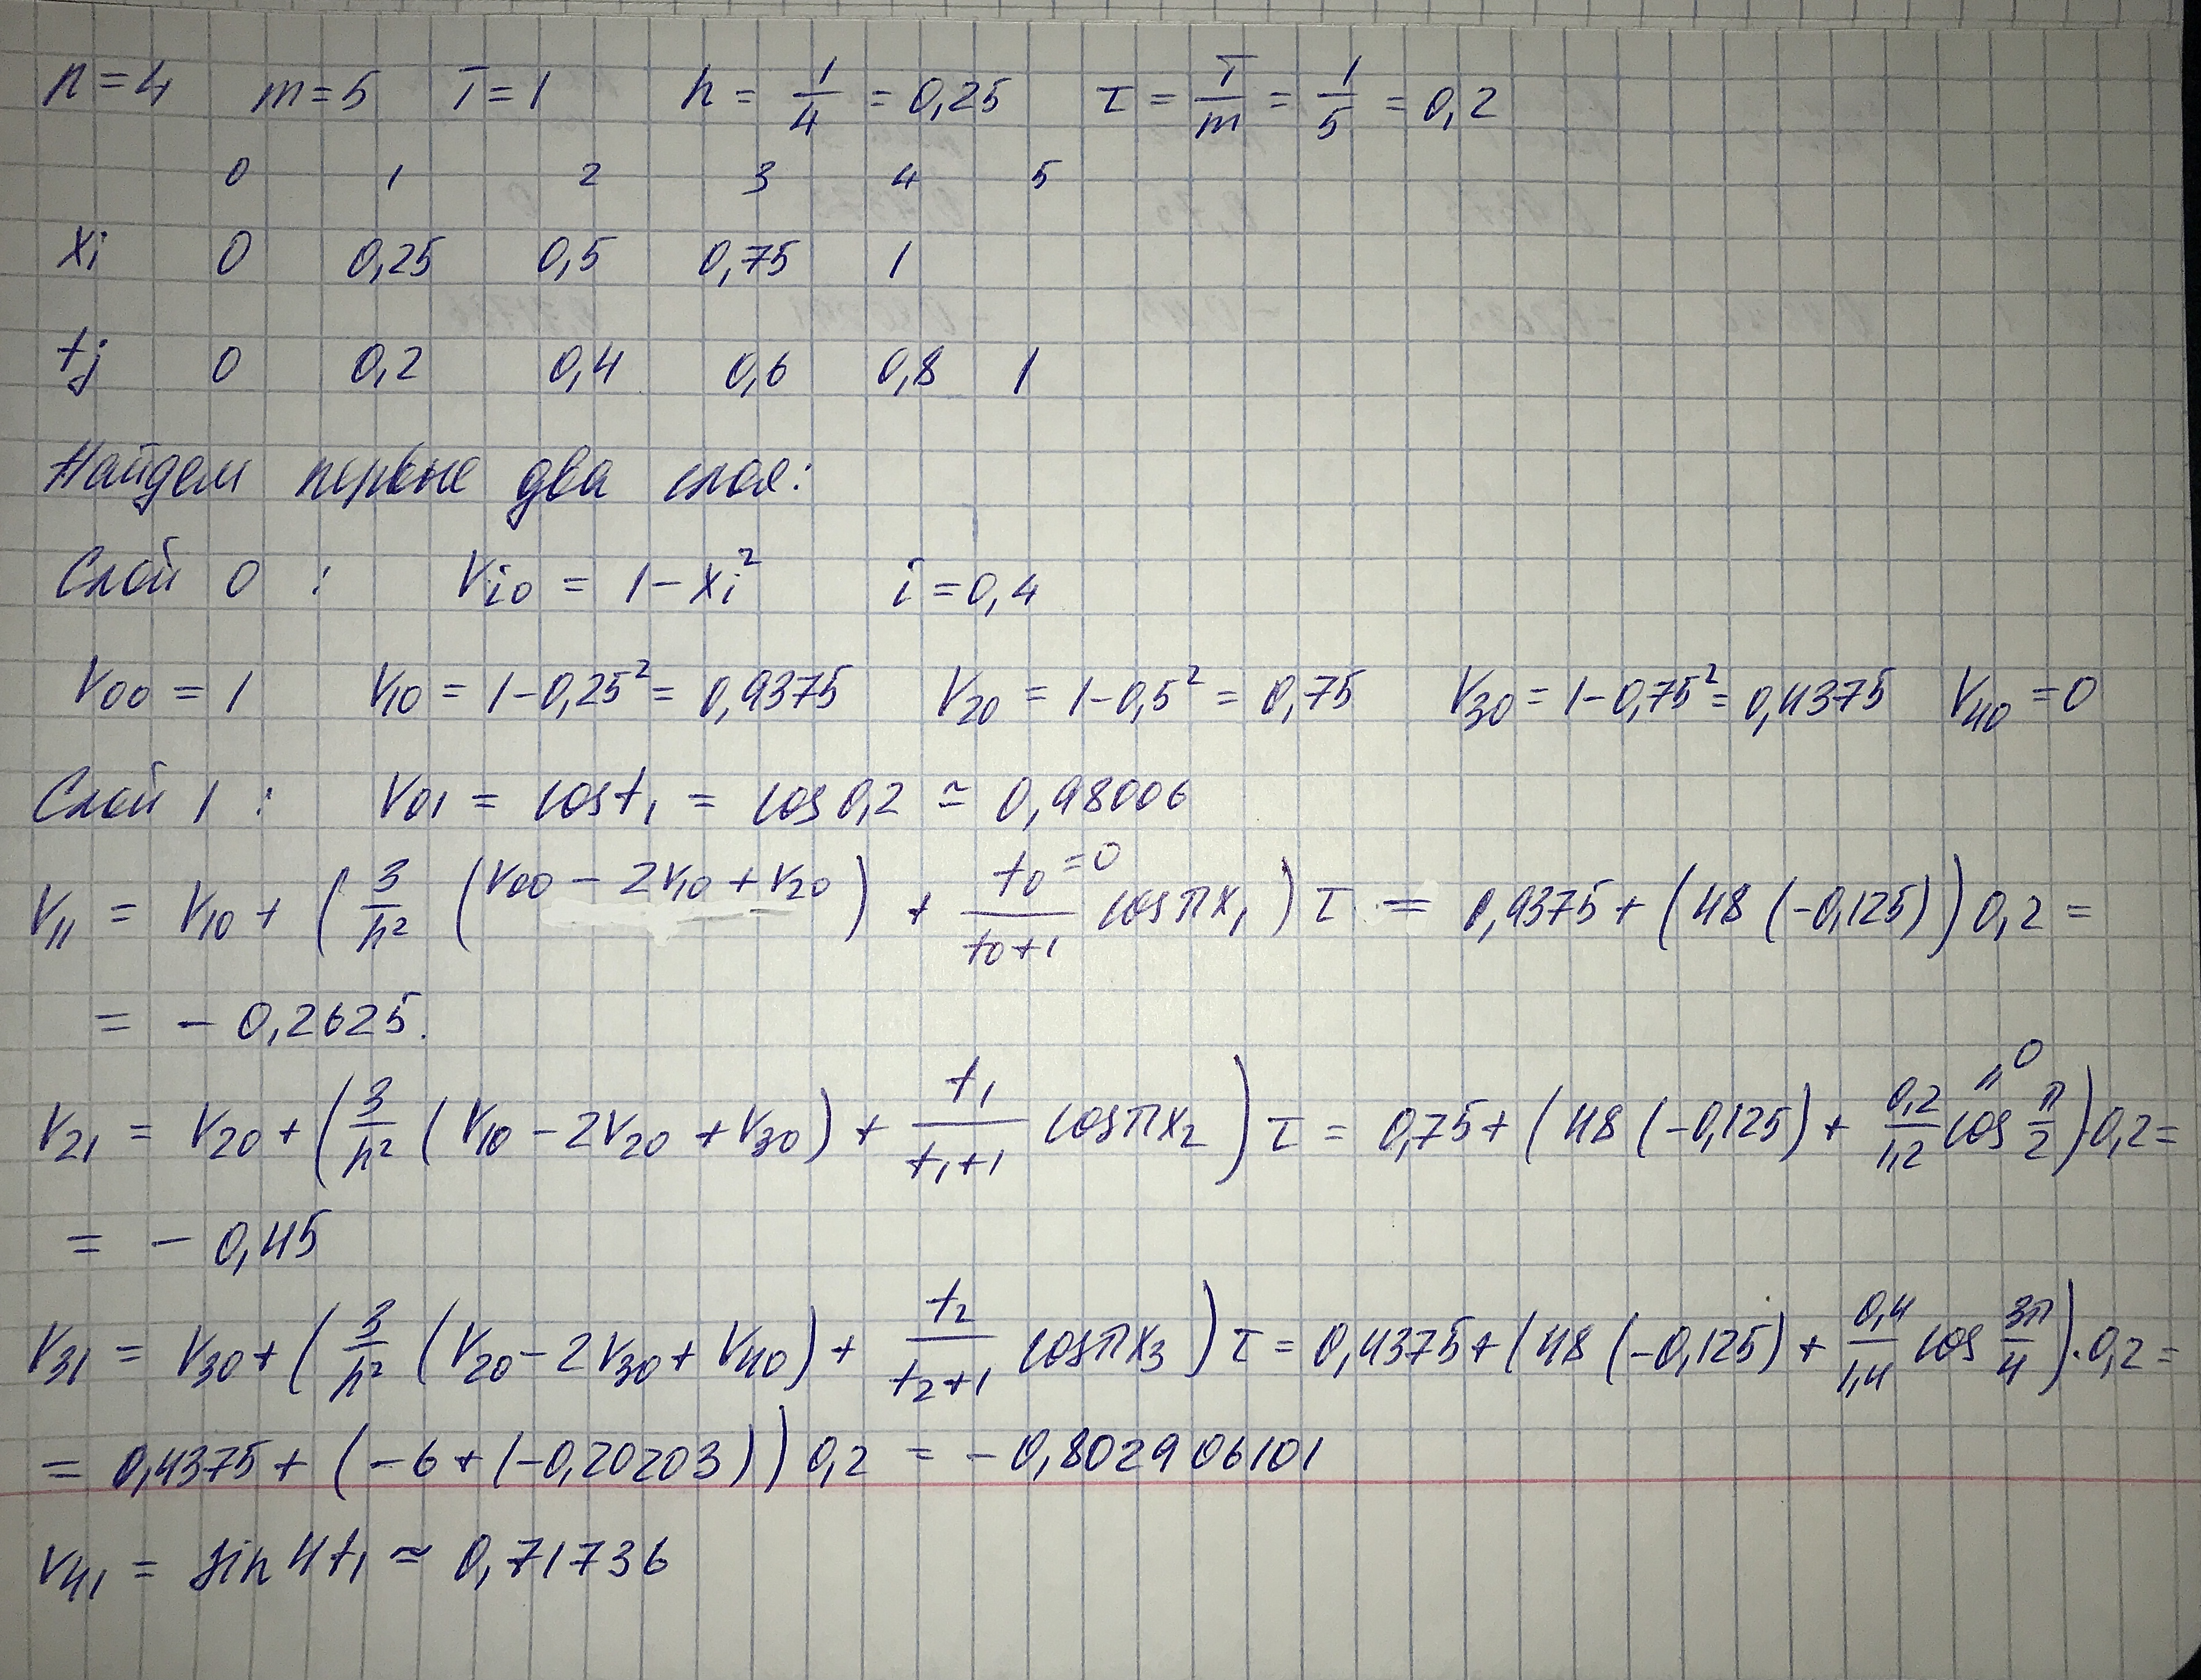
\includegraphics[scale=0.06]{calculus1}}
		\end{figure}
	\end{frame}

	\begin{frame}
		\frametitle{Проверим корректность вычислений программы}
		\begin{figure}[h]
			\center{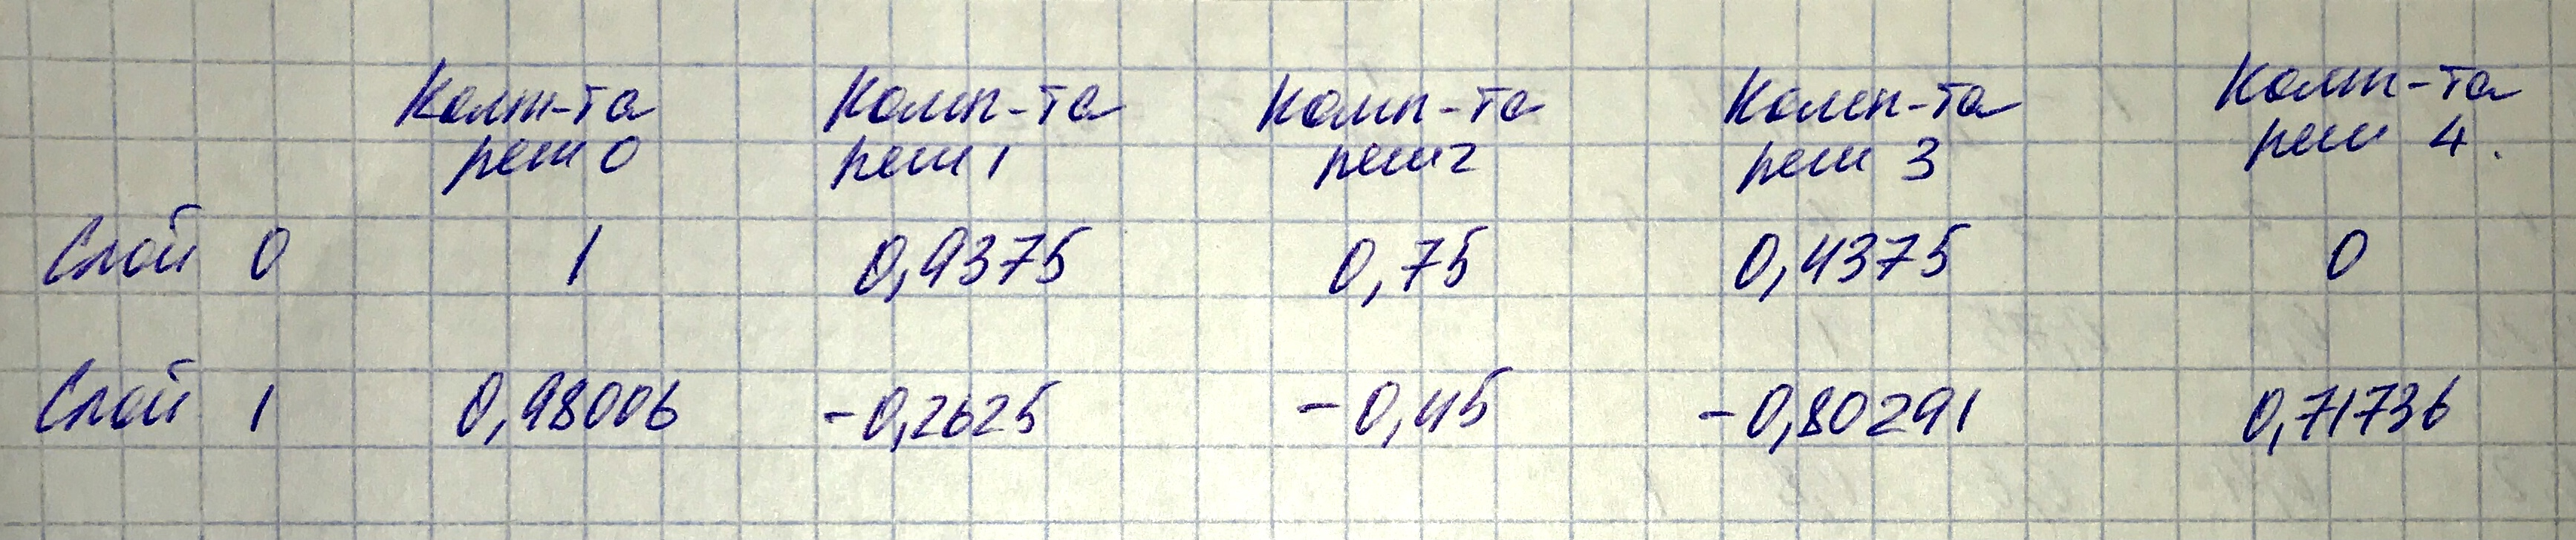
\includegraphics[scale=0.06]{calculus2}}
		\end{figure}

		\begin{figure}[h]
			\center{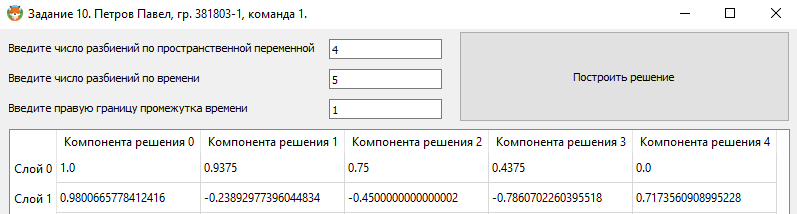
\includegraphics[scale=0.5]{layers01}}
		\end{figure}
	\end{frame}

	\begin{frame}
		\frametitle{Свойства схемы}
		Явная схема сходится условно, то есть сходимость наблюдается только тогда, когда $\tau < \frac{h^2}{2\gamma^2} = \frac{h^2}{6}$.
		\newline 
		Так как в программе вводятся параметры $n, m, T$, то найдём для них соотношение, при котором наблюдается сходимость.
		\[ \frac{T}{m} < \frac{1}{6n^2} \]
		\[ \frac{m}{T} > 6n^2 \]
		\[ m > 6Tn^2 \]
	\end{frame}

\end{document}
